%!TEX root = ../cv.tex
% -*- root: ../cv.tex -*-

%-------------------------------------------------------------------------------
%	SECTION TITLE
%-------------------------------------------------------------------------------
\cvsection{Experience}


%-------------------------------------------------------------------------------
%	CONTENT
%-------------------------------------------------------------------------------
\begin{cventries}
%---------------------------------------------------------
  \cventry
    {Deep Learning} % Job title
    {} % Organization
    {} % Location
    {Level: B-} % Date(s)
    {
      \begin{cvitems} % Description(s) of tasks/responsibilities
        \item {Research on Classification to Recognize Driver Environments and Status using Deep Learning}
        \item {Steering Wheel Region Segmentation using Deconv Net}
        \item {DNN Learning and Applying using TensorFlow}
      \end{cvitems}
    }

%---------------------------------------------------------
  \cventry
    {Computer Vision and Pattern Recognition} % Job title
    {} % Organization
    {} % Location
    {Level: B+} % Date(s)
    {
      \begin{cvitems} % Description(s) of tasks/responsibilities
        \item {Develop for Mobile Augmented Reality using Local Feature Tracking \\
               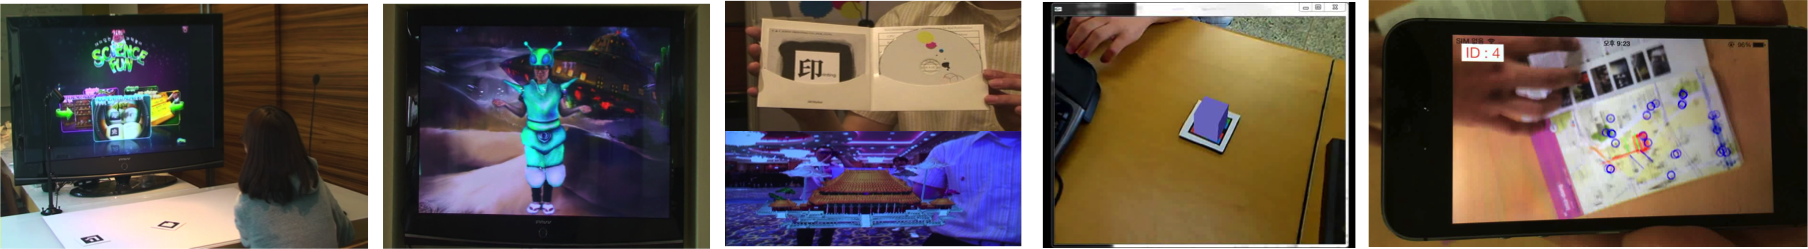
\includegraphics[width=\linewidth]{cv/resources/ar.png} }
          \begin{itemize}
            \item {Develop a feature point filtering algorithm for high performance and speed}
          \end{itemize}
        \item {Research on Recognizing Bare Hands using Depth Camera \\
               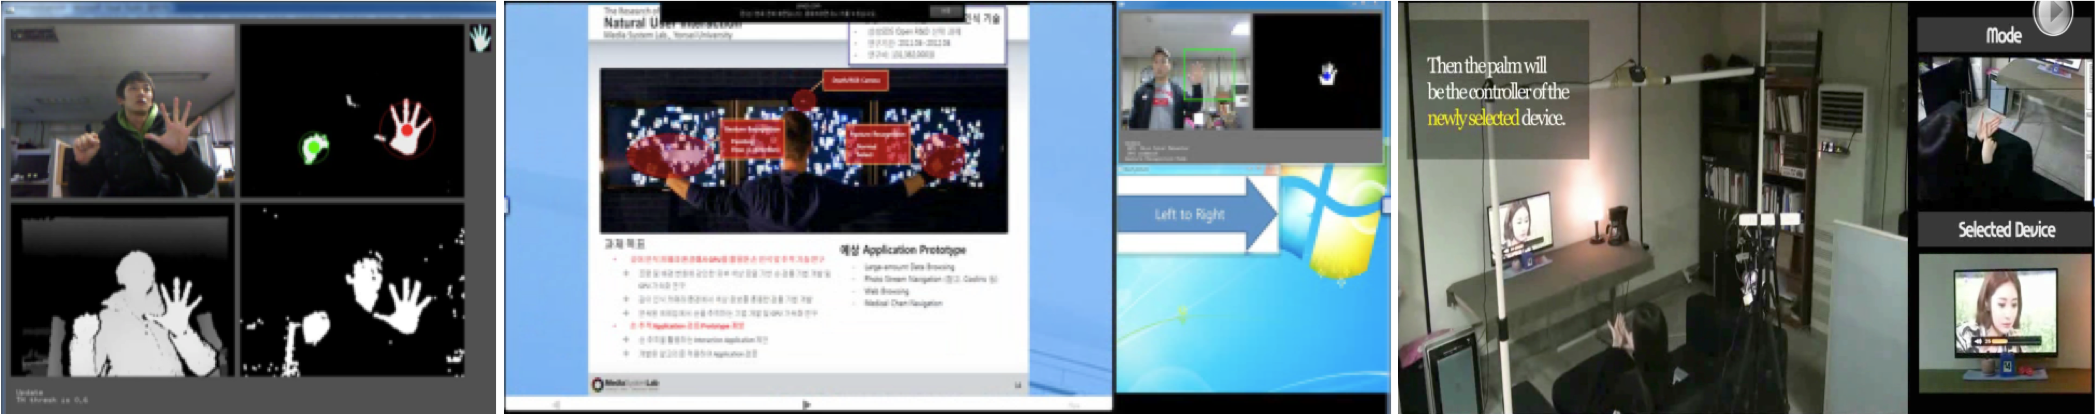
\includegraphics[width=\linewidth]{cv/resources/hand.png} }
        \item {Spoke/Steering Wheel Region Tracking for Driver Status Monitoring}
      \end{cvitems}
    }

%---------------------------------------------------------
  \cventry
    {Device Fast Prototyping} % Job title
    {} % Organization
    {} % Location
    {Level: A+} % Date(s)
    {
      \begin{cvitems} % Description(s) of tasks/responsibilities
        \item {Developing Spatial AR Environment using $360^{\circ}$ Steerable Projector \\
          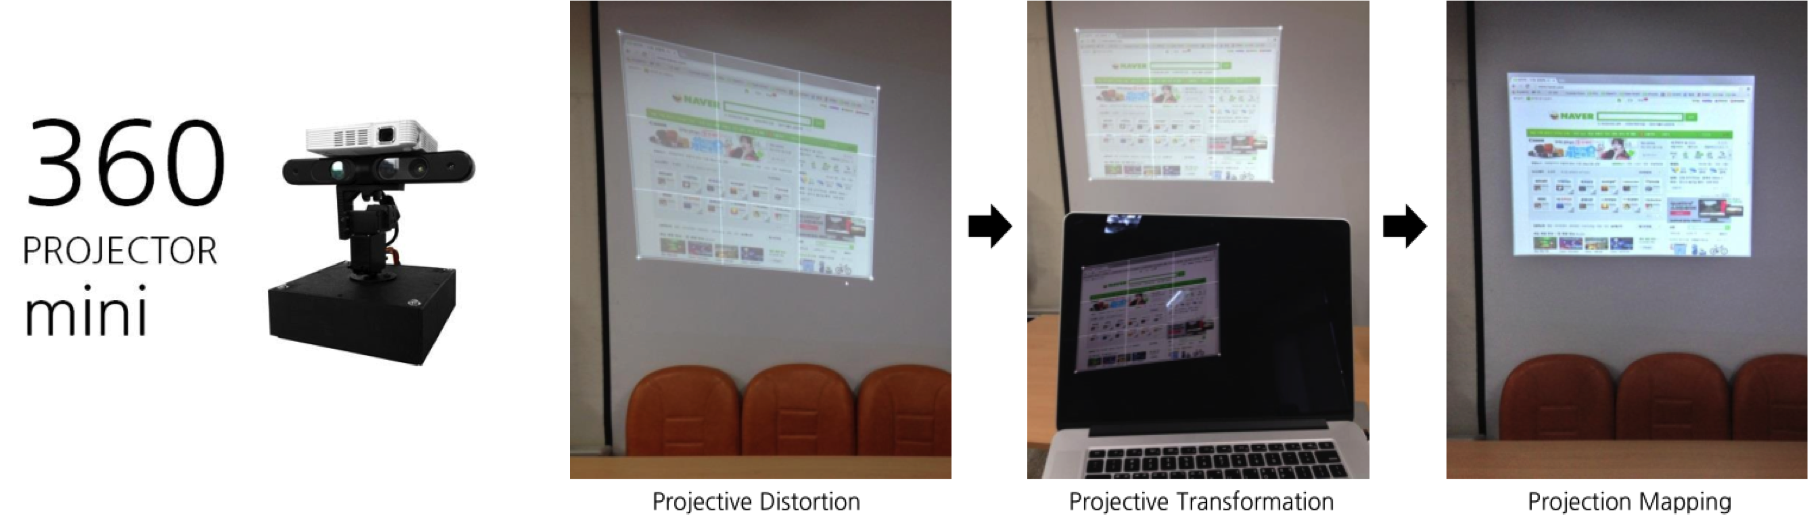
\includegraphics[width=\linewidth]{cv/resources/pervasiveAR.png}
          \begin{itemize}
              \item {Pico Projector, Small Depth Camera, Arduino based Pan-Tilt Motor System}
              \item {Research a computer vision based projecting image rectification algorithm for pan-tilt projector}
          \end{itemize}
        }
        \item {Pen-type Interface which Augments Information on the Surface \\
          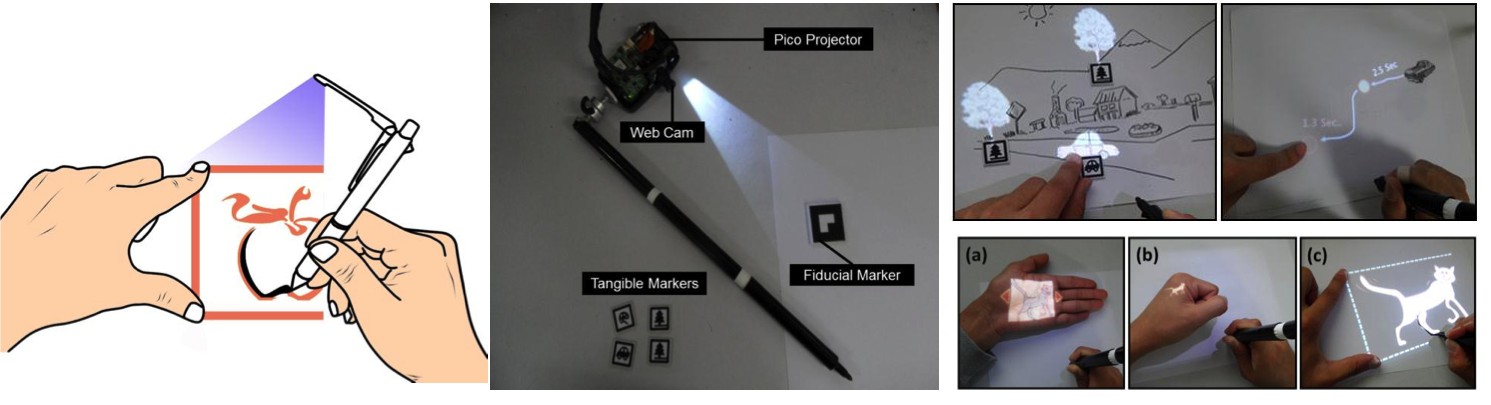
\includegraphics[width=\linewidth, height=40mm]{cv/resources/augpen.png}
          \begin{itemize}
            \item {Pico Projector, Small Web Camera, Fiducial Marker}
            \item {Research on Interating Technology with 2D Contents and Bare Hand}
          \end{itemize}
        }
        \item {Sensor-based Gestural Interfaces \\
          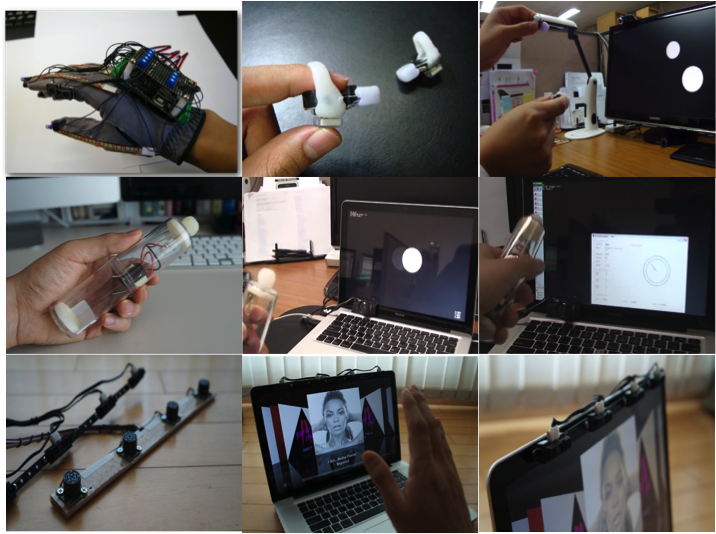
\includegraphics[width=\linewidth]{cv/resources/gesturedevices.png}
          \begin{itemize}
            \item {Developing Various Types of Sensor Interfaces to Recognize Hand Interaction}
            \item {Developing Gesture Interface using IR Blob, Flex Sensor, Gyro Sensor, Lidar Sensor, etc}
          \end{itemize}
        }
      \end{cvitems} 
    }
\end{cventries}
